% Gabarit pandoc des corrigés publiés (brut et guidé). Contenu sans marque ni nom de site.
% Compilation : lualatex (latexmk -lualatex).
% Le Markdown reste la source unique : ne pas éditer ce fichier .tex à la main.
\documentclass[11pt,a4paper]{article}

% --- Moteur, polices (Latin Modern) et langue ---------------------------------
\usepackage{iftex}
\ifLuaTeX\else\errmessage{Ce document se compile avec lualatex}\fi
\usepackage{amsmath,amssymb,mathtools}
\usepackage{fontspec}
% mathrm=sym : \mathrm prend ses glyphes dans la police mathématique (ℓ, μ, Ω), comme KaTeX.
\usepackage[math-style=TeX,bold-style=TeX,mathrm=sym]{unicode-math}
% Repli pour les glyphes absents de Latin Modern (indices et exposants Unicode,
% flèches, filets des schémas en texte, symboles) : DejaVu, puis Latin Modern Math
% (ℓ, lettres mathématiques Unicode des légendes).
\directlua{
  luaotfload.add_fallback("repliTexte", {"DejaVuSerif:mode=harf;", "DejaVuSans:mode=harf;", "file:latinmodern-math.otf:mode=harf;"})
  luaotfload.add_fallback("repliMono", {"DejaVuSansMono:mode=harf;", "DejaVuSans:mode=harf;", "file:latinmodern-math.otf:mode=harf;"})
}
\setmainfont{Latin Modern Roman}[RawFeature={fallback=repliTexte}]
\setsansfont{Latin Modern Sans}[RawFeature={fallback=repliTexte}]
\setmonofont{Latin Modern Mono}[RawFeature={fallback=repliMono}]
\setmathfont{Latin Modern Math}
\usepackage[french]{babel}
\frenchsetup{SmallCapsFigTabCaptions=false}

% --- Mise en page --------------------------------------------------------------
\usepackage[a4paper,margin=2.2cm,headheight=14pt,footskip=1.2cm]{geometry}
\usepackage{microtype}
\setlength{\emergencystretch}{4em}
\tolerance=1500
\setlength{\parindent}{0pt}
\setlength{\parskip}{0.55\baselineskip plus 2pt minus 1pt}
\usepackage{xcolor}
% Gris nommés : babel-french rend « ! » actif dans le document.
\definecolor{gris2}{gray}{0.98}
\definecolor{gris3}{gray}{0.97}
\definecolor{gris5}{gray}{0.95}
\definecolor{gris35}{gray}{0.65}
\definecolor{gris40}{gray}{0.60}
\definecolor{gris45}{gray}{0.55}
\definecolor{gris50}{gray}{0.50}
\definecolor{gris55}{gray}{0.45}
\definecolor{gris60}{gray}{0.40}
\definecolor{gris65}{gray}{0.35}
\definecolor{gris70}{gray}{0.30}
\definecolor{gris80}{gray}{0.20}
\definecolor{gris85}{gray}{0.15}
\usepackage{graphicx}
\usepackage{float}
\usepackage{caption}
\captionsetup{font=small,labelformat=empty,justification=centering}
\usepackage{booktabs,longtable,array,multirow,calc}
\usepackage{siunitx}
\sisetup{locale=FR}
\usepackage[version=4]{mhchem}
\usepackage{listings}
\usepackage{fancyhdr}
\usepackage{lastpage}
\usepackage[most]{tcolorbox}
\usepackage{enumitem}
\setlist{nosep,leftmargin=*,topsep=2pt}
\usepackage[hidelinks,unicode]{hyperref}
\usepackage{bookmark}
\hypersetup{pdftitle={Mines-Ponts PSI — Maths 2 2026},pdfauthor={Rédigé par IA},pdfcreator={LaTeX},pdfsubject={Corrigé brut}}
\usepackage{xurl}

% --- Pandoc : listes, tableaux, figures ----------------------------------------
\providecommand{\passthrough}[1]{#1}
\providecommand{\tightlist}{\setlength{\itemsep}{0pt}\setlength{\parskip}{0pt}}

\makeatletter
\def\maxwidth{\ifdim\Gin@nat@width>\linewidth\linewidth\else\Gin@nat@width\fi}
\def\maxheight{\ifdim\Gin@nat@height>0.55\textheight 0.55\textheight\else\Gin@nat@height\fi}
\makeatother
\setkeys{Gin}{width=\maxwidth,height=\maxheight,keepaspectratio}
\setcounter{secnumdepth}{-\maxdimen}
\providecommand{\pandocbounded}[1]{#1}

% --- Code (listings) -----------------------------------------------------------
\lstset{
  basicstyle=\ttfamily\small,
  columns=fullflexible,
  keepspaces=true,
  breaklines=true,
  breakatwhitespace=false,
  postbreak=\mbox{\textcolor{gris50}{$\hookrightarrow$}\space},
  frame=single,
  rulecolor=\color{gris35},
  framesep=4pt,
  xleftmargin=5pt,xrightmargin=5pt,
  backgroundcolor=\color{gris3},
  keywordstyle=\bfseries,
  commentstyle=\color{gris65},
  stringstyle=\color{gris80},
  showstringspaces=false,
  tabsize=4,
  extendedchars=true,
  aboveskip=6pt,belowskip=6pt,
}

% --- Macros des corrigés (KaTeX ↔ LaTeX) ---------------------------------------
% Les corrigés sont écrits pour KaTeX : on définit ici ce que KaTeX connaît et
% que LaTeX n'a pas, sans jamais retoucher le Markdown.
\providecommand{\R}{\mathbb{R}}
\providecommand{\N}{\mathbb{N}}
\providecommand{\Z}{\mathbb{Z}}
\providecommand{\Q}{\mathbb{Q}}
\providecommand{\C}{\mathbb{C}}
\providecommand{\dd}{\mathrm{d}}
\providecommand{\llbracket}{\lBrack}
\providecommand{\rrbracket}{\rBrack}
\providecommand{\lBrace}{\lbrace}
\providecommand{\rBrace}{\rbrace}
\providecommand{\Box}{\square}
\providecommand{\Diamond}{\lozenge}
\providecommand{\varnothing}{\emptyset}
\providecommand{\argmax}{\operatorname*{arg\,max}}
\providecommand{\argmin}{\operatorname*{arg\,min}}
\renewcommand{\leq}{\leqslant}
\renewcommand{\geq}{\geqslant}

% Équation hors texte : réduite à la largeur de la ligne si elle déborde.
\newsavebox{\boiteequation}
\newcommand{\equationajustee}[1]{%
  \sbox{\boiteequation}{$\displaystyle #1$}%
  \ifdim\wd\boiteequation>\linewidth
    \[\resizebox{\linewidth}{!}{\usebox{\boiteequation}}\]%
  \else
    \[#1\]%
  \fi}

% --- Encadrés pédagogiques (sobres, lisibles en noir et blanc) -----------------
\tcbset{
  encadre/.style={
    enhanced,breakable,sharp corners,
    colback=white,colframe=gris55,
    boxrule=0.4pt,leftrule=2.2pt,
    left=6pt,right=6pt,top=3pt,bottom=3pt,
    before skip=6pt,after skip=6pt,
    fonttitle=\bfseries\small,coltitle=black,
    attach title to upper,after title={\quad},
    parbox=false,
  }
}
\newtcolorbox{indication}[1]{encadre,colframe=gris45,colback=gris2,title={Indication~#1}}
\newtcolorbox{methode}{encadre,colframe=gris70,title={Méthode}}
\newtcolorbox{piege}{encadre,colframe=gris85,boxrule=0.8pt,leftrule=2.2pt,title={Piège}}
\newtcolorbox{jury}{encadre,colframe=gris60,colback=gris5,title={Jury}}
\newtcolorbox{encadrenote}{encadre,colframe=gris40}

% --- Titres de section ---------------------------------------------------------
\usepackage{titlesec}
\titleformat{\section}{\Large\bfseries}{}{0pt}{}
\titleformat{\subsection}{\large\bfseries}{}{0pt}{}
\titleformat{\subsubsection}{\normalsize\bfseries}{}{0pt}{}
\titlespacing*{\section}{0pt}{14pt plus 4pt minus 2pt}{6pt}
\titlespacing*{\subsection}{0pt}{10pt plus 3pt minus 2pt}{4pt}
\titlespacing*{\subsubsection}{0pt}{8pt plus 2pt minus 2pt}{2pt}

% --- En-tête et pied de page ---------------------------------------------------
\pagestyle{fancy}
\fancyhf{}
\fancyhead[L]{\small\textsc{Corrigé brut} · Mines-Ponts PSI}
\fancyhead[R]{\small Maths 2 2026}
\fancyfoot[L]{\footnotesize Corrigé rédigé par IA, non officiel}
\fancyfoot[R]{\footnotesize \thepage\,/\,\pageref*{LastPage}}
\renewcommand{\headrulewidth}{0.4pt}
\renewcommand{\footrulewidth}{0pt}
\fancypagestyle{plain}{\fancyhf{}\fancyfoot[R]{\footnotesize \thepage\,/\,\pageref*{LastPage}}\fancyfoot[L]{\footnotesize Corrigé rédigé par IA, non officiel}\renewcommand{\headrulewidth}{0pt}}

\begin{document}
\thispagestyle{plain}
\begin{center}
  {\small\scshape Corrigé brut}\par\smallskip
  {\LARGE\bfseries Mines-Ponts PSI — Maths 2 2026\par}\medskip
  {\large Mines-Ponts · PSI · Maths 2 · 2026\par}
\end{center}
\vspace{2pt}\hrule\vspace{8pt}

\emph{Corrigé rédigé par IA, non officiel. Signalez toute erreur.}

Probabilité qu'un entier choisi au hasard et uniformément dans \([\![1;n]\!]\) soit sans facteur à la puissance \(k\). Durée 3 heures, calculatrice interdite.

\hypertarget{partie-1-calcul-de-la-somme-sum_n1inftyfrac1n2x2}{%
\section{\texorpdfstring{Partie 1 : Calcul de la somme \(\sum_{n=1}^{+\infty}\frac{1}{n^2+x^2}\)}{Partie 1 : Calcul de la somme \textbackslash sum\_\{n=1\}\^{}\{+\textbackslash infty\}\textbackslash frac\{1\}\{n\^{}2+x\^{}2\}}}\label{partie-1-calcul-de-la-somme-sum_n1inftyfrac1n2x2}}

\hypertarget{question-1}{%
\subsection{Question 1}\label{question-1}}

Soit \(\theta\in\mathbb{R}\setminus2\pi\mathbb{Z}\) et \(n\in{\mathbb{N}}^*\). Pour \(t\in[0;1]\), on a \(|e^{i\theta}t|=t\le1\).

Si l'on avait \(e^{i\theta}t=1\), on aurait \(t=|e^{i\theta}t|=1\), puis \(e^{i\theta}=1\), soit \(\theta\in2\pi\mathbb{Z}\) : c'est exclu.

Donc \(1-e^{i\theta}t\ne0\) sur \([0;1]\), et l'intégrande est continue sur \([0;1]\).

La raison \(q=e^{i\theta}t\) étant différente de \(1\), la somme géométrique finie donne
\equationajustee{\begin{aligned}
e^{i\theta}\,\frac{1-(e^{i\theta}t)^n}{1-e^{i\theta}t}&=e^{i\theta}\sum_{j=0}^{n-1}(e^{i\theta}t)^j\\
&=\sum_{k=1}^{n}e^{ik\theta}t^{k-1}.
\end{aligned}}
On intègre sur \([0;1]\) par linéarité de l'intégrale (somme finie), avec \(\int_0^1t^{k-1}\,\mathrm{d}t=\frac1k\) :
\equationajustee{\boxed{\int_0^1e^{i\theta}\,\frac{1-(e^{i\theta}t)^n}{1-e^{i\theta}t}\,\mathrm{d}t=\sum_{k=1}^{n}\frac{e^{ik\theta}}{k}.}}

\hypertarget{question-2}{%
\subsection{Question 2}\label{question-2}}

\textbf{Minoration du dénominateur.} Pour \(u\in[0;1]\),
\equationajustee{\begin{aligned}
|1-e^{i\theta}u|^2&=1-2u\cos\theta+u^2\\
&=(u-\cos\theta)^2+\sin^2\theta.
\end{aligned}}
Si \(\sin\theta\ne0\), on en tire \(|1-e^{i\theta}u|\ge|\sin\theta|\).

Si \(\sin\theta=0\), comme \(\theta\notin2\pi\mathbb{Z}\), on a \(\cos\theta=-1\), d'où \(|1-e^{i\theta}u|=1+u\ge1\).

En posant \(c_\theta=\min(1,|\sin\theta|)>0\), on obtient dans tous les cas
\equationajustee{(\star)\qquad\forall u\in[0;1],\ |1-e^{i\theta}u|\ge c_\theta.}

\begin{figure}[H]
\centering
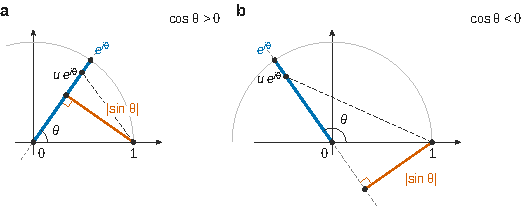
\includegraphics{figures/q2-distance-segment.pdf}
\caption*{Figure 1 --- Distance du point 1 au segment d'extrémités 0 et
e\^{}\{iθ\} : elle est au moins \textbar sin θ\textbar, distance de 1 à
la droite portant le segment, que le pied de la perpendiculaire soit sur
le segment (a) ou sur son prolongement (b)}
\end{figure}

\textbf{Convergence.} D'après \((\star)\), la fonction \(t\mapsto\frac{e^{i\theta}}{1-e^{i\theta}t}\) est continue sur \([0;1]\) ; notons \(I(\theta)\) son intégrale. Par la question 1,
\equationajustee{\sum_{k=1}^{n}\frac{e^{ik\theta}}{k}-I(\theta)=-\int_0^1\frac{e^{i\theta}(e^{i\theta}t)^n}{1-e^{i\theta}t}\,\mathrm{d}t.}
On majore le module de l'intégrale par l'intégrale du module (on ne compare que des modules, qui sont réels), puis on utilise \((\star)\) :
\equationajustee{(\star\star)\qquad\begin{aligned}
\left|\sum_{k=1}^{n}\frac{e^{ik\theta}}{k}-I(\theta)\right|&\le\int_0^1\frac{t^n}{c_\theta}\,\mathrm{d}t\\
&=\frac{1}{c_\theta(n+1)}.
\end{aligned}}
Ce majorant tend vers \(0\) quand \(n\to+\infty\). Les sommes partielles convergent : \textbf{la série \(\sum_{k\ge1}\frac{e^{ik\theta}}{k}\) converge} et
\equationajustee{\boxed{\sum_{k=1}^{+\infty}\frac{e^{ik\theta}}{k}=\int_0^1\frac{e^{i\theta}}{1-e^{i\theta}t}\,\mathrm{d}t.}}

\hypertarget{question-3}{%
\subsection{Question 3}\label{question-3}}

Soit \(\theta\in\,]0;\pi[\). Les sommes partielles de \(\sum e^{ik\theta}/k\) convergent dans \(\mathbb{C}\), donc leurs parties imaginaires convergent vers la partie imaginaire de la limite. La série \(\sum_{k\ge1}\frac{\sin(k\theta)}{k}\) converge donc.

La partie imaginaire d'une intégrale de fonction complexe étant l'intégrale de la partie imaginaire,
\equationajustee{\sum_{k=1}^{+\infty}\frac{\sin(k\theta)}{k}=\int_0^1\operatorname{Im}\left(\frac{e^{i\theta}}{1-e^{i\theta}t}\right)\mathrm{d}t.}
Or, en multipliant par le conjugué du dénominateur,
\equationajustee{\begin{aligned}
\frac{e^{i\theta}}{1-e^{i\theta}t}&=\frac{e^{i\theta}(1-e^{-i\theta}t)}{|1-e^{i\theta}t|^2}\\
&=\frac{e^{i\theta}-t}{1-2t\cos\theta+t^2},
\end{aligned}}
donc
\equationajustee{\operatorname{Im}\left(\frac{e^{i\theta}}{1-e^{i\theta}t}\right)=\frac{\sin\theta}{1-2t\cos\theta+t^2}.}

\textbf{La fonction \(u_\theta\) est bien définie.} Pour \(t\in[0;1]\), on a \(1-t\cos\theta>0\). En effet, si \(\cos\theta\le0\), ce nombre vaut au moins \(1\) ; sinon, il vaut au moins \(1-\cos\theta>0\).

Donc \(u_\theta\) est définie et de classe \(\mathcal C^1\) sur \([0;1]\).

Posons \(f(t)=\frac{t\sin\theta}{1-t\cos\theta}\). Alors
\equationajustee{\begin{aligned}
f'(t)&=\frac{\sin\theta(1-t\cos\theta)+t\sin\theta\cos\theta}{(1-t\cos\theta)^2}\\
&=\frac{\sin\theta}{(1-t\cos\theta)^2},
\end{aligned}}
puis
\equationajustee{\begin{aligned}
u_\theta'(t)&=\frac{f'(t)}{1+f(t)^2}\\
&=\frac{\sin\theta}{(1-t\cos\theta)^2+t^2\sin^2\theta}\\
&=\frac{\sin\theta}{1-2t\cos\theta+t^2}.
\end{aligned}}
Ainsi
\equationajustee{\begin{aligned}
\sum_{k=1}^{+\infty}\frac{\sin(k\theta)}{k}&=\int_0^1u_\theta'(t)\,\mathrm{d}t\\
&=u_\theta(1)-u_\theta(0)\\
&=\operatorname{Arctan}\left(\frac{\sin\theta}{1-\cos\theta}\right).
\end{aligned}}

Avec \(\theta/2\in\,]0;\pi/2[\), les formules de l'angle moitié donnent
\equationajustee{\begin{aligned}
\frac{\sin\theta}{1-\cos\theta}&=\frac{2\sin(\theta/2)\cos(\theta/2)}{2\sin^2(\theta/2)}\\
&=\frac{\cos(\theta/2)}{\sin(\theta/2)}\\
&=\tan\left(\frac{\pi-\theta}{2}\right).
\end{aligned}}
Comme \(\frac{\pi-\theta}{2}\in\,]0;\pi/2[\,\subset\,]-\pi/2;\pi/2[\), intervalle sur lequel \(\operatorname{Arctan}(\tan y)=y\), on conclut. Pour tout \(\theta\in\,]0;\pi[\) :
\equationajustee{\boxed{\sum_{k=1}^{+\infty}\frac{\sin(k\theta)}{k}=\frac{\pi-\theta}{2}.}}

\hypertarget{question-4}{%
\subsection{Question 4}\label{question-4}}

Posons \(s_n(t)=\frac{\cos(nt)}{n^2}\) pour \(n\ge1\). Chaque \(s_n\) est continue sur \(\mathbb{R}\).

Pour tout \(t\in\mathbb{R}\), \(|s_n(t)|\le\frac1{n^2}\), et la série \(\sum\frac1{n^2}\) converge (série de Riemann d'exposant \(2>1\), résultat du cours).

La série \(\sum s_n\) converge donc \textbf{normalement sur \(\mathbb{R}\)}, donc simplement : \(S\) est bien définie sur \(\mathbb{R}\).

La convergence normale sur \(\mathbb{R}\) entraîne la convergence uniforme sur \(\mathbb{R}\). Les \(s_n\) étant continues, le théorème de continuité de la somme d'une série de fonctions donne : \textbf{\(S\) est continue sur \(\mathbb{R}\)}.

\hypertarget{question-5}{%
\subsection{Question 5}\label{question-5}}

Pour \(\theta=0\), les deux membres valent \(S(0)\). Soit \(\theta\in\,]0;\pi[\) et \(a\in\,]0;\theta[\).

\textbf{Convergence uniforme sur \([a;\theta]\).} La fonction \(\sin\), concave sur \([0;\pi]\), atteint son minimum sur \([a;\theta]\) en une borne.

Ainsi, pour \(t\in[a;\theta]\), \(\sin t\ge m\) avec \(m=\min(\sin a,\sin\theta)>0\). En posant \(c=\min(1,m)>0\), on a donc \(c_t\ge c\).

La majoration \((\star\star)\), l'inégalité \(|\operatorname{Im}z|\le|z|\) et la valeur \(\operatorname{Im}I(t)=\frac{\pi-t}{2}\) (question 3) donnent, pour tout \(t\in[a;\theta]\) et tout \(n\ge1\),
\equationajustee{\left|\sum_{k=1}^{n}\frac{\sin(kt)}{k}-\frac{\pi-t}{2}\right|\le\frac{1}{c(n+1)}.}
Le majorant ne dépend pas de \(t\) et tend vers \(0\) : la série de fonctions continues \(\sum\frac{\sin(kt)}{k}\) converge uniformément sur le segment \([a;\theta]\) vers \(t\mapsto\frac{\pi-t}{2}\).

\textbf{Intégration terme à terme sur \([a;\theta]\).} Le théorème d'intégration terme à terme d'une série de fonctions continues uniformément convergente sur un segment donne
\equationajustee{\sum_{n=1}^{+\infty}\int_a^\theta\frac{\sin(nt)}{n}\,\mathrm{d}t=\int_a^\theta\frac{\pi-t}{2}\,\mathrm{d}t.}
Or \(\int_a^\theta\frac{\sin(nt)}{n}\,\mathrm{d}t=\frac{\cos(na)-\cos(n\theta)}{n^2}\). Les séries \(\sum\frac{\cos(na)}{n^2}\) et \(\sum\frac{\cos(n\theta)}{n^2}\) convergent (question 4), d'où
\equationajustee{S(a)-S(\theta)=\left(\frac{\pi\theta}{2}-\frac{\theta^2}{4}\right)-\left(\frac{\pi a}{2}-\frac{a^2}{4}\right).}

\textbf{Limite \(a\to0^+\).} \(S\) est continue en \(0\) (question 4). En faisant tendre \(a\) vers \(0\), on obtient
\equationajustee{S(0)-S(\theta)=\frac{\pi\theta}{2}-\frac{\theta^2}{4}.}
Pour tout \(\theta\in[0;\pi[\) :
\equationajustee{\boxed{S(\theta)=\frac{\theta^2}{4}-\frac{\pi\theta}{2}+S(0).}}
Les deux membres étant continus sur \(\mathbb{R}\), l'égalité \textbf{s'étend à \(\theta=\pi\)} par passage à la limite \(\theta\to\pi^-\) ; on l'utilise en question 8.

\begin{figure}[H]
\centering
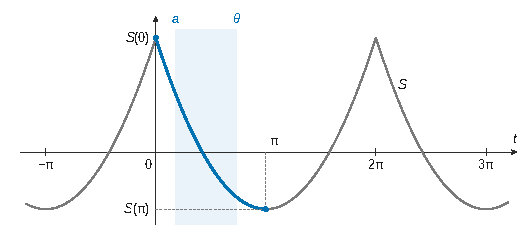
\includegraphics{figures/q5-fonction-s.pdf}
\caption*{Figure 2 --- La fonction S, paire et 2π-périodique : sur l'intervalle de
0 à π (arc bleu) elle coïncide avec t²/4 − πt/2 + S(0), obtenue sur un
segment de a à θ qui évite 0, puis par a → 0}
\end{figure}

\hypertarget{question-6}{%
\subsection{Question 6}\label{question-6}}

Fixons \(x\in\mathbb{R}\) et posons \(u_n(t)=\frac{\cos(nt)}{n^2(n^2+x^2)}\). Chaque \(u_n\) est de classe \(\mathcal C^2\) sur \(\mathbb{R}\), avec
\equationajustee{\begin{aligned}
u_n'(t)&=-\frac{\sin(nt)}{n(n^2+x^2)},\\
u_n''(t)&=-\frac{\cos(nt)}{n^2+x^2}.
\end{aligned}}
Comme \(n^2+x^2\ge n^2\), on a pour tout \(t\in\mathbb{R}\) :
\equationajustee{\begin{aligned}
|u_n(t)|&\le\frac1{n^4},\\
|u_n'(t)|&\le\frac1{n^3},\\
|u_n''(t)|&\le\frac1{n^2}.
\end{aligned}}
Les séries \(\sum u_n\), \(\sum u_n'\) et \(\sum u_n''\) convergent donc normalement, donc uniformément et en particulier simplement, sur \(\mathbb{R}\).

Le théorème de dérivation terme à terme (classe \(\mathcal C^2\)) s'applique, car ses trois hypothèses sont satisfaites :

\begin{itemize}
\tightlist
\item
  les \(u_n\) sont de classe \(\mathcal C^2\) sur \(\mathbb{R}\) ;
\item
  les séries \(\sum u_n\) et \(\sum u_n'\) convergent simplement sur \(\mathbb{R}\) ;
\item
  la série \(\sum u_n''\) converge uniformément sur \(\mathbb{R}\).
\end{itemize}

Donc \textbf{\(g_x\) est de classe \(\mathcal C^2\) sur \(\mathbb{R}\)}, et l'on dérive terme à terme :
\equationajustee{\begin{aligned}
g_x'(t)&=-\sum_{n=1}^{+\infty}\frac{\sin(nt)}{n(n^2+x^2)},\\
g_x''(t)&=-\sum_{n=1}^{+\infty}\frac{\cos(nt)}{n^2+x^2}.
\end{aligned}}
Par linéarité (séries convergentes),
\equationajustee{\begin{aligned}
g_x''(t)-x^2g_x(t)&=-\sum_{n=1}^{+\infty}\cos(nt)\,\frac{n^2+x^2}{n^2(n^2+x^2)}\\
&=-\sum_{n=1}^{+\infty}\frac{\cos(nt)}{n^2}.
\end{aligned}}
Pour tout \(t\in\mathbb{R}\) :
\equationajustee{\boxed{g_x''(t)-x^2g_x(t)=-S(t).}}

\hypertarget{question-7}{%
\subsection{Question 7}\label{question-7}}

Soit \(x\ne0\). Cherchons \(P(t)=at^2+bt+c\). Alors
\equationajustee{P''(t)-x^2P(t)=-ax^2t^2-bx^2t+(2a-cx^2).}
Il suffit que ces coefficients soient ceux de \(-\frac{t^2}{4}+\frac{\pi t}{2}-S(0)\), c'est-à-dire
\equationajustee{\begin{aligned}
-ax^2&=-\frac14,\\
-bx^2&=\frac\pi2,\\
2a-cx^2&=-S(0).
\end{aligned}}
Puisque \(x\ne0\), on prend \(a=\frac1{4x^2}\), \(b=-\frac{\pi}{2x^2}\) et \(c=\frac{2a+S(0)}{x^2}\), d'où le candidat
\equationajustee{\boxed{P(t)=\frac{t^2}{4x^2}-\frac{\pi t}{2x^2}+\frac{1}{2x^4}+\frac{S(0)}{x^2}.}}

\textbf{Vérification.} On a, pour tout \(t\in\mathbb{R}\),
\equationajustee{\begin{aligned}
P'(t)&=\frac{t}{2x^2}-\frac{\pi}{2x^2}=\frac{t-\pi}{2x^2},\\
P''(t)&=\frac{1}{2x^2},
\end{aligned}}
d'où
\equationajustee{\begin{aligned}
P''(t)-x^2P(t)&=\frac{1}{2x^2}-\left(\frac{t^2}{4}-\frac{\pi t}{2}+\frac{1}{2x^2}+S(0)\right)\\
&=-\frac{t^2}{4}+\frac{\pi t}{2}-S(0).
\end{aligned}}
Le polynôme \(P\), de degré \(2\) (coefficient dominant \(\frac1{4x^2}\ne0\)), est donc bien solution de \((E_x)\) sur \(\mathbb{R}\).

\hypertarget{question-8}{%
\subsection{Question 8}\label{question-8}}

\textbf{Dérivées premières.} Soit \(x\in\mathbb{R}\). Dans l'expression de \(g_x'\) obtenue à la question 6, tous les termes sont nuls en \(0\) et en \(\pi\), car \(\sin0=\sin(n\pi)=0\). Donc
\equationajustee{\boxed{\begin{aligned}
g_x'(0)&=0,\\
g_x'(\pi)&=0.
\end{aligned}}}

\textbf{Résolution sur \([0;\pi]\).} Soit \(x\ne0\). Par la question 5, étendue à \(\pi\) par continuité, on a pour tout \(t\in[0;\pi]\)
\equationajustee{-S(t)=-\frac{t^2}{4}+\frac{\pi t}{2}-S(0).}
La question 6 montre donc que la restriction de \(g_x\) à l'intervalle \([0;\pi]\) est solution de \((E_x)\) sur cet intervalle (et non sur \(\mathbb{R}\) : hors de \([0;\pi]\), \(-S\) n'est plus ce polynôme).

L'équation homogène \(y''-x^2y=0\) est linéaire à coefficients constants. Son équation caractéristique \(r^2-x^2=0\) a deux racines réelles \textbf{distinctes} \(x\) et \(-x\), précisément parce que \(x\ne0\).

Les solutions de l'équation homogène sur \([0;\pi]\) sont donc les fonctions \(t\mapsto Ae^{xt}+Be^{-xt}\), avec \((A,B)\in{\mathbb{R}}^2\).

Les solutions de \((E_x)\) sur \([0;\pi]\) s'obtiennent en leur ajoutant la solution particulière \(P\) de la question 7. Il existe donc \((A,B)\in{\mathbb{R}}^2\) tel que
\equationajustee{\forall t\in[0;\pi],\ g_x(t)=P(t)+Ae^{xt}+Be^{-xt}.}

\textbf{Constantes.} Pour \(t\in[0;\pi]\),
\equationajustee{g_x'(t)=\frac{t-\pi}{2x^2}+Axe^{xt}-Bxe^{-xt}.}
La condition \(g_x'(0)=0\) s'écrit \(-\frac{\pi}{2x^2}+x(A-B)=0\), et la condition \(g_x'(\pi)=0\) s'écrit \(x(Ae^{\pi x}-Be^{-\pi x})=0\). Comme \(x\ne0\) :
\equationajustee{\begin{aligned}
A-B&=\frac{\pi}{2x^3},\\
B&=Ae^{2\pi x}.
\end{aligned}}
Comme \(x\ne0\), on a \(1-e^{2\pi x}\ne0\), et
\equationajustee{\begin{aligned}
A&=\frac{\pi}{2x^3(1-e^{2\pi x})},\\
B&=\frac{\pi e^{2\pi x}}{2x^3(1-e^{2\pi x})},\\
A+B&=\frac{\pi(1+e^{2\pi x})}{2x^3(1-e^{2\pi x})}.
\end{aligned}}

\textbf{Calcul de \(g_x''(0)\).} On dérive deux fois l'expression de \(g_x\) sur \([0;\pi]\) :
\equationajustee{\begin{aligned}
g_x''(0)&=P''(0)+x^2(A+B)\\
&=\frac{1}{2x^2}+\frac{\pi(1+e^{2\pi x})}{2x(1-e^{2\pi x})}.
\end{aligned}}
En multipliant numérateur et dénominateur par \(e^{-2\pi x}\) :
\equationajustee{\begin{aligned}
\frac{1+e^{2\pi x}}{1-e^{2\pi x}}&=\frac{e^{-2\pi x}+1}{e^{-2\pi x}-1}\\
&=-\frac{1+e^{-2\pi x}}{1-e^{-2\pi x}},
\end{aligned}}
d'où
\equationajustee{\boxed{g_x''(0)=-\frac{\pi}{2x}\times\frac{1+e^{-2\pi x}}{1-e^{-2\pi x}}+\frac{1}{2x^2}.}}

\hypertarget{question-9}{%
\subsection{Question 9}\label{question-9}}

Soit \(x\ne0\). Par la question 6 en \(t=0\), \(g_x''(0)=-\sum_{n\ge1}\frac{1}{n^2+x^2}\). Avec la question 8, en multipliant par \(-2x^2\) :
\equationajustee{\sum_{n=1}^{+\infty}\frac{2x^2}{n^2+x^2}=\pi x\,\frac{1+e^{-2\pi x}}{1-e^{-2\pi x}}-1.}
Or, en multipliant haut et bas par \(e^{2\pi x}\) (avec \(e^{2\pi x}\ne1\)) :
\equationajustee{\begin{aligned}
\frac{1+e^{-2\pi x}}{1-e^{-2\pi x}}&=\frac{e^{2\pi x}+1}{e^{2\pi x}-1}\\
&=1+\frac{2}{e^{2\pi x}-1}.
\end{aligned}}
Donc
\equationajustee{\sum_{n=1}^{+\infty}\frac{2x^2}{n^2+x^2}=\pi x+\frac{2\pi x}{e^{2\pi x}-1}-1,}
c'est-à-dire, pour tout \(x\in{\mathbb{R}}^*\),
\equationajustee{\boxed{\frac{2\pi x}{e^{2\pi x}-1}=1-\pi x+\sum_{n=1}^{+\infty}\frac{2x^2}{n^2+x^2}.}}

\hypertarget{partie-2-duxe9veloppement-en-suxe9rie-entiuxe8re-de-xmapstofracxex-1-et-applications}{%
\section{\texorpdfstring{Partie 2 : Développement en série entière de \(x\mapsto\frac{x}{e^x-1}\) et applications}{Partie 2 : Développement en série entière de x\textbackslash mapsto\textbackslash frac\{x\}\{e\^{}x-1\} et applications}}\label{partie-2-duxe9veloppement-en-suxe9rie-entiuxe8re-de-xmapstofracxex-1-et-applications}}

\hypertarget{question-10}{%
\subsection{Question 10}\label{question-10}}

Soient \(x\in\,]-1;1[\), \(N\in\mathbb{N}\) et \(n\in{\mathbb{N}}^*\). Posons \(q=-\frac{x^2}{n^2}\).

On a \(q\le0\), donc \(q\ne1\), et \(1-q=\frac{n^2+x^2}{n^2}\). La somme géométrique \textbf{finie} donne
\equationajustee{\begin{aligned}
\frac1{n^2}\sum_{k=0}^{N}q^k&=\frac1{n^2}\cdot\frac{1-q^{N+1}}{1-q}\\
&=\frac{1}{x^2+n^2}-\frac{q^{N+1}}{x^2+n^2}.
\end{aligned}}
Et
\equationajustee{\frac{q^{N+1}}{x^2+n^2}=(-1)^{N+1}\frac{1}{x^2+n^2}\times\frac{x^{2N+2}}{n^{2N+2}}=R_{N,n}(x).}
D'où
\equationajustee{\boxed{\frac{1}{x^2+n^2}=\left(\frac1{n^2}\sum_{k=0}^{N}\left(\frac{-x^2}{n^2}\right)^k\right)+R_{N,n}(x).}}

Comme \(x^2+n^2\ge1\), on a \(|R_{N,n}(x)|\le\frac{|x|^{2N+2}}{n^{2N+2}}\). La série \(\sum_n n^{-(2N+2)}\) converge (série de Riemann d'exposant \(2N+2\ge2\)), de somme \(\zeta(2N+2)\). Par comparaison de séries à termes positifs, la série \(\sum_n|R_{N,n}(x)|\) converge, et
\equationajustee{\boxed{\sum_{n=1}^{+\infty}|R_{N,n}(x)|\le\zeta(2N+2)\,|x|^{2N+2}.}}

\hypertarget{question-11}{%
\subsection{Question 11}\label{question-11}}

\textbf{Limite de \(\zeta\).} Pour \(s\ge2\) et \(n\ge2\),
\equationajustee{\frac1{n^s}=\frac1{n^2}\cdot\frac1{n^{s-2}}\le\frac{1}{2^{s-2}}\cdot\frac1{n^2}.}
En sommant ces inégalités entre termes de séries convergentes,
\equationajustee{\begin{aligned}
0\le\zeta(s)-1&=\sum_{n=2}^{+\infty}\frac1{n^s}\\
&\le\frac{\zeta(2)-1}{2^{s-2}}.
\end{aligned}}
Ce majorant tend vers \(0\) quand \(s\to+\infty\), donc \(\lim_{s\to+\infty}\zeta(s)=1\). En particulier, la suite \((\zeta(2N+2))_{N\in\mathbb{N}}\) est bornée.

\textbf{Sommation.} Soit \(x\in\,]-1;1[\). En multipliant l'identité de la question 10 par \(x^2\) et en posant \(j=k+1\) :
\equationajustee{\frac{x^2}{x^2+n^2}=\sum_{j=1}^{N+1}(-1)^{j+1}\frac{x^{2j}}{n^{2j}}+x^2R_{N,n}(x).}
Chacune des séries \(\sum_n n^{-2j}\) converge (somme \(\zeta(2j)\)), ainsi que \(\sum_nR_{N,n}(x)\) (question 10). La somme sur \(j\) étant \textbf{finie}, on peut sommer sur \(n\) par linéarité :
\equationajustee{\begin{aligned}
\sum_{n=1}^{+\infty}\frac{x^2}{x^2+n^2}&=\sum_{j=1}^{N+1}(-1)^{j+1}\zeta(2j)x^{2j}\\
&\quad+x^2\sum_{n=1}^{+\infty}R_{N,n}(x).
\end{aligned}}
Par la question 10, le dernier terme est majoré en module par \(x^2\zeta(2N+2)|x|^{2N+2}\). Ce majorant tend vers \(0\) quand \(N\to+\infty\), car \(\zeta(2N+2)\) est bornée et \(|x|<1\).

Les sommes partielles de la série \(\sum_{k\ge1}(-1)^{k+1}\zeta(2k)x^{2k}\) convergent donc. Pour tout \(x\in\,]-1;1[\) :
\equationajustee{\boxed{\begin{aligned}{}&\sum_{n=1}^{+\infty}\frac{x^2}{x^2+n^2}\\
&\quad=\sum_{k=1}^{+\infty}(-1)^{k+1}\zeta(2k)\,x^{2k}.
\end{aligned}}}

\hypertarget{question-12}{%
\subsection{Question 12}\label{question-12}}

Soit \(X\in\,]-2\pi;2\pi[\) avec \(X\ne0\). Posons \(x=\frac{X}{2\pi}\), de sorte que \(x\in\,]-1;1[\setminus\{0\}\).

On réserve la lettre \(X\) à la variable de \(h\) et la lettre \(x\) à celle des questions 9 et 11. La question 9 s'écrit
\equationajustee{h(X)=1-\frac X2+2\sum_{n=1}^{+\infty}\frac{x^2}{n^2+x^2},}
et la question 11 donne
\equationajustee{\begin{aligned}
h(X)&=1-\frac X2+2\sum_{k=1}^{+\infty}(-1)^{k+1}\zeta(2k)\frac{X^{2k}}{(2\pi)^{2k}}\\
&=1-\frac X2+\sum_{k=1}^{+\infty}(-1)^{k+1}\frac{\zeta(2k)}{2^{2k-1}\pi^{2k}}X^{2k}.
\end{aligned}}
En \(X=0\), cas exclu de la question 9, les deux membres valent \(1\) par définition de \(h\). Donc, pour tout \(x\in\,]-2\pi;2\pi[\) :
\equationajustee{\boxed{h(x)=1-\frac12x+\sum_{k=1}^{+\infty}(-1)^{k+1}\frac{\zeta(2k)}{2^{2k-1}\pi^{2k}}x^{2k}.}}
Cette série entière converge en tout point de \(]-2\pi;2\pi[\), donc son rayon est au moins \(2\pi\) : \textbf{\(h\) est développable en série entière} (sur \(]-2\pi;2\pi[\)).

La somme d'une série entière \(\sum a_mx^m\) est de classe \(\mathcal C^\infty\) sur l'intervalle ouvert de convergence, avec \(a_m=\frac{h^{(m)}(0)}{m!}\). Donc \(b_m=m!\,a_m\), et
\equationajustee{\boxed{\begin{aligned}
b_0&=1,\\
b_1&=-\frac12,\\
b_{2k}&=(-1)^{k+1}\frac{(2k)!\,\zeta(2k)}{2^{2k-1}\pi^{2k}}\ \ (k\ge1),\\
b_{2k+1}&=0\ \ (k\ge1).
\end{aligned}}}

\hypertarget{question-13}{%
\subsection{Question 13}\label{question-13}}

Sur \(]-2\pi;2\pi[\), \(h(x)=\sum_{k\ge0}\frac{b_k}{k!}x^k\), série entière de rayon \(R_1\ge2\pi\) (question 12).

Pour tout réel \(x\), posons \(\varphi(x)=\sum_{j\ge0}\frac{x^j}{(j+1)!}\). Cette série entière a un rayon infini, et la série de l'exponentielle donne \(\varphi(x)=\frac{e^x-1}{x}\) si \(x\ne0\), \(\varphi(0)=1\).

Rappelons le théorème sur le produit de Cauchy. Soient \(\sum\alpha_kx^k\) et \(\sum\beta_jx^j\) deux séries entières de rayons \(R_1\) et \(R_2\), et \(c_n=\sum_{k=0}^{n}\alpha_k\beta_{n-k}\).

Alors la série entière \(\sum c_nx^n\) a un rayon au moins \(\min(R_1,R_2)\), et pour \(|x|<\min(R_1,R_2)\) sa somme est le produit des deux sommes.

Ici \(\min(R_1,+\infty)\ge2\pi\), donc pour tout \(x\in\,]-2\pi;2\pi[\) :
\equationajustee{h(x)\varphi(x)=\sum_{n=0}^{+\infty}c_nx^n,}
avec
\equationajustee{c_n=\sum_{k=0}^{n}\frac{b_k}{k!}\cdot\frac{1}{(n-k+1)!}.}
Or \(h(x)\varphi(x)=\frac{x}{e^x-1}\times\frac{e^x-1}{x}=1\) si \(x\ne0\), et \(h(0)\varphi(0)=1\). La fonction \(h\varphi\) est donc constante égale à \(1\) sur \(]-2\pi;2\pi[\).

Par unicité des coefficients d'un développement en série entière sur un voisinage de \(0\), on obtient \(c_0=1\) et \(c_n=0\) pour \(n\ge1\). Pour tout \(n\in{\mathbb{N}}^*\) :
\equationajustee{\boxed{\sum_{k=0}^{n}\frac{b_k}{k!\,(n+1-k)!}=0.}}

\hypertarget{question-14}{%
\subsection{Question 14}\label{question-14}}

Pour \(n=2\) :
\equationajustee{\begin{aligned}
\frac{b_0}{0!\,3!}+\frac{b_1}{1!\,2!}+\frac{b_2}{2!\,1!}&=\frac16-\frac14+\frac{b_2}{2}\\
&=0,
\end{aligned}}
d'où \(\boxed{b_2=\frac16}\).

Pour \(n=4\), avec \(b_3=0\) (question 12) :
\equationajustee{\begin{aligned}
0&=\frac{b_0}{0!\,5!}+\frac{b_1}{1!\,4!}+\frac{b_2}{2!\,3!}+\frac{b_4}{4!\,1!}\\
&=\frac1{120}-\frac1{48}+\frac1{72}+\frac{b_4}{24}\\
&=\frac{6-15+10}{720}+\frac{b_4}{24},
\end{aligned}}
d'où \(b_4=-\frac{24}{720}\), soit \(\boxed{b_4=-\frac1{30}}\).

Par la question 12, avec \(k=1\) puis \(k=2\) :
\equationajustee{\begin{aligned}
b_2&=\frac{2!\,\zeta(2)}{2\pi^2}=\frac{\zeta(2)}{\pi^2},\\
b_4&=-\frac{4!\,\zeta(4)}{2^3\pi^4}=-\frac{3\zeta(4)}{\pi^4}.
\end{aligned}}
Donc
\equationajustee{\boxed{\begin{aligned}
\zeta(2)&=\frac{\pi^2}{6},\\
\zeta(4)&=\frac{\pi^4}{90}.
\end{aligned}}}

\hypertarget{partie-3-probabilituxe9-quun-entier-naturel-choisi-au-hasard-et-uniformuxe9ment-dans-1n-soit-sans-facteur-uxe0-la-puissance-k}{%
\section{\texorpdfstring{Partie 3 : Probabilité qu'un entier naturel choisi au hasard et uniformément dans \([\![1;n]\!]\) soit sans facteur à la puissance \(k\)}{Partie 3 : Probabilité qu'un entier naturel choisi au hasard et uniformément dans {[}\textbackslash!{[}1;n{]}\textbackslash!{]} soit sans facteur à la puissance k}}\label{partie-3-probabilituxe9-quun-entier-naturel-choisi-au-hasard-et-uniformuxe9ment-dans-1n-soit-sans-facteur-uxe0-la-puissance-k}}

\hypertarget{question-15}{%
\subsection{Question 15}\label{question-15}}

Soit \((x_1,\dots,x_r)\in{\mathbb{R}}^r\). Pour \(1\le m\le r\), notons
\equationajustee{\Sigma_m^{(r)}=\sum_{i_1<\dots<i_m}x_{i_1}\cdots x_{i_m}\qquad(\text{indices dans }[\![1;r]\!]),}
avec \(\Sigma_0^{(r)}=1\) et \(\Sigma_m^{(r)}=0\) si \(m>r\). Montrons par récurrence sur \(r\ge1\) que \(\prod_{i=1}^{r}(1+x_i)=\sum_{m=0}^{r}\Sigma_m^{(r)}\).

Pour \(r=1\) : \(1+x_1=\Sigma_0^{(1)}+\Sigma_1^{(1)}\).

Hérédité. On sépare les \(m\)-uplets \(1\le i_1<\dots<i_m\le r+1\) selon que \(i_m=r+1\) ou \(i_m\le r\). Pour \(1\le m\le r+1\), cela donne
\equationajustee{\Sigma_m^{(r+1)}=\Sigma_m^{(r)}+x_{r+1}\Sigma_{m-1}^{(r)}.}
Avec l'hypothèse de récurrence et \(\Sigma_{r+1}^{(r)}=0\) :
\equationajustee{\begin{aligned}
\sum_{m=0}^{r+1}\Sigma_m^{(r+1)}&=1+\sum_{m=1}^{r+1}\Sigma_m^{(r)}+x_{r+1}\sum_{m=1}^{r+1}\Sigma_{m-1}^{(r)}\\
&=\sum_{m=0}^{r}\Sigma_m^{(r)}+x_{r+1}\sum_{m=0}^{r}\Sigma_m^{(r)}\\
&=(1+x_{r+1})\prod_{i=1}^{r}(1+x_i).
\end{aligned}}
D'où, pour tout \(r\in{\mathbb{N}}^*\) :
\equationajustee{\boxed{\begin{aligned}{}&\prod_{i=1}^{r}(1+x_i)\\
&\quad=1+\sum_{m=1}^{r}\left(\sum_{1\le i_1<\dots<i_m\le r}x_{i_1}x_{i_2}\cdots x_{i_m}\right).
\end{aligned}}}
(Dans l'énoncé, la condition \(1\le i_1<\dots<i_m\le r\) porte sur les \(m\)-uplets d'indices \((i_1,\dots,i_m)\).)

\hypertarget{question-16}{%
\subsection{Question 16}\label{question-16}}

Les deux égalités sont des égalités de fonctions sur \(\Omega\) ; soit \(\omega\in\Omega\) une issue.

Si \(\omega\in A\), alors \(\mathbf 1_{\bar A}(\omega)=0=1-\mathbf 1_A(\omega)\). Si \(\omega\notin A\), alors \(\mathbf 1_{\bar A}(\omega)=1=1-\mathbf 1_A(\omega)\). Donc \(\boxed{\mathbf 1_{\bar A}=1-\mathbf 1_A}\).

Les nombres \(\mathbf 1_{A_i}(\omega)\) valent \(0\) ou \(1\).

Leur produit vaut \(1\) si et seulement si tous valent \(1\), c'est-à-dire si \(\omega\in A_1\cap\dots\cap A_m\) ; il vaut \(0\) sinon.

Donc \(\boxed{\mathbf 1_{A_1}\mathbf 1_{A_2}\cdots\mathbf 1_{A_m}=\mathbf 1_{A_1\cap A_2\cap\dots\cap A_m}}\).

\hypertarget{question-17}{%
\subsection{Question 17}\label{question-17}}

Par De Morgan, \(\overline{A_1\cup\dots\cup A_r}=\bar A_1\cap\dots\cap\bar A_r\). La question 16 donne donc
\equationajustee{\begin{aligned}
\mathbf 1_{A_1\cup\dots\cup A_r}&=1-\prod_{i=1}^{r}\mathbf 1_{\bar A_i}\\
&=1-\prod_{i=1}^{r}(1-\mathbf 1_{A_i}).
\end{aligned}}
On applique la question 15 en chaque \(\omega\) avec \(x_i=-\mathbf 1_{A_i}(\omega)\), puis la question 16 :
\equationajustee{\begin{aligned}{}&\prod_{i=1}^{r}(1-\mathbf 1_{A_i})\\
&\quad=1+\sum_{m=1}^{r}(-1)^m\sum_{1\le i_1<\dots<i_m\le r}\mathbf 1_{A_{i_1}\cap\dots\cap A_{i_m}}.
\end{aligned}}
D'où
\equationajustee{\begin{aligned}{}&\mathbf 1_{A_1\cup\dots\cup A_r}\\
&\quad=\sum_{m=1}^{r}(-1)^{m+1}\sum_{1\le i_1<\dots<i_m\le r}\mathbf 1_{A_{i_1}\cap\dots\cap A_{i_m}}.
\end{aligned}}
Ces indicatrices sont des variables aléatoires bornées, donc d'espérance finie. On prend l'espérance, par linéarité (somme finie) et avec \(E(\mathbf 1_B)=P(B)\) :
\equationajustee{\boxed{\begin{aligned}{}&P(A_1\cup\dots\cup A_r)\\
&\quad=\sum_{m=1}^{r}(-1)^{m+1}\left(\sum_{1\le i_1<\dots<i_m\le r}P(A_{i_1}\cap\dots\cap A_{i_m})\right).
\end{aligned}}}

\hypertarget{question-18}{%
\subsection{Question 18}\label{question-18}}

Un entier \(m\in[\![1;n]\!]\) n'est pas dans \(S_n(k)\) si et seulement s'il existe \(j\in[\![1;r]\!]\) tel que \(p_j^k\mid m\), c'est-à-dire \(m\in A_n(p_j^k)\). Ainsi \([\![1;n]\!]\setminus S_n(k)=\bigcup_{i=1}^{r}A_n(p_i^k)\), et
\equationajustee{\boxed{q_n(k)=1-P_n\left(\bigcup_{i=1}^{r}A_n(p_i^k)\right).}}
(Tester \(p_1,\dots,p_r\) suffit : si \(p\) premier vérifie \(p^k\mid m\) avec \(m\le n\), alors \(p\le m\le n\).

Ainsi \(q_n(k)\) est bien la probabilité que l'entier tiré soit sans facteur à la puissance \(k\).)

La question 17 donne
\equationajustee{\begin{aligned}
q_n(k)&=1-\sum_{m=1}^{r}(-1)^{m+1}\sum_{1\le i_1<\dots<i_m\le r}P_n\left(\bigcap_{\ell=1}^{m}A_n(p_{i_\ell}^k)\right)\\
&=1+\sum_{m=1}^{r}\sum_{1\le i_1<\dots<i_m\le r}(-1)^mP_n\left(\bigcap_{\ell=1}^{m}A_n(p_{i_\ell}^k)\right).
\end{aligned}}
Soit \(j\in[\![1;n]\!]\) tel que \(p_{i_\ell}^k\mid j\) pour tout \(\ell\). Les \(p_{i_\ell}\) sont des nombres premiers \textbf{deux à deux distincts} : la décomposition en facteurs premiers de \(j\) contient chacun d'eux avec un exposant au moins \(k\).

Donc \(p_{i_1}^k\cdots p_{i_m}^k\mid j\) ; la réciproque est immédiate. Ainsi \(\bigcap_\ell A_n(p_{i_\ell}^k)=A_n(p_{i_1}^k\cdots p_{i_m}^k)\), et
\equationajustee{\boxed{\begin{aligned}{}&q_n(k)\\
&\quad=1+\sum_{m=1}^{r}\sum_{1\le i_1<i_2<\dots<i_m\le r}(-1)^m\,P_n\left(A_n\left(p_{i_1}^kp_{i_2}^k\cdots p_{i_m}^k\right)\right).
\end{aligned}}}

\hypertarget{question-19}{%
\subsection{Question 19}\label{question-19}}

Les multiples de \(d\) dans \([\![1;n]\!]\) sont \(d,2d,\dots,\lfloor n/d\rfloor d\). La probabilité \(P_n\) étant uniforme, \(P_n(A_n(d))=\frac1n\left\lfloor\frac nd\right\rfloor\).

Pour \(1\le i_1<\dots<i_m\le r\), posons \(D=p_{i_1}\cdots p_{i_m}\). Alors \(p_{i_1}^k\cdots p_{i_m}^k=D^k\) et \(\mu(D)=(-1)^m\).

L'application \(\{i_1<\dots<i_m\}\mapsto p_{i_1}\cdots p_{i_m}\) (pour \(m\ge1\)) est injective, par unicité de la décomposition en facteurs premiers.

Son image est l'ensemble \(\mathcal D\) des entiers \(D>1\) sans facteur carré dont tous les facteurs premiers sont parmi \(p_1,\dots,p_r\). Le terme \(1\) s'écrit \(\frac1n\mu(1)\lfloor n/1^k\rfloor\). Ainsi
\equationajustee{q_n(k)=\frac1n\sum_{D\in\{1\}\cup\mathcal D}\mu(D)\left\lfloor\frac{n}{D^k}\right\rfloor.}
Soit \(d\ge1\) hors de \(\{1\}\cup\mathcal D\).

\begin{itemize}
\tightlist
\item
  Ou bien \(d\) a un facteur carré, et \(\mu(d)=0\).
\item
  Ou bien \(d\) a un facteur premier \(p\notin\{p_1,\dots,p_r\}\), donc \(p>n\). Alors \(d^k\ge d\ge p>n\), d'où \(\lfloor n/d^k\rfloor=0\).
\end{itemize}

Ces termes sont nuls : la série ci-dessous n'a qu'un nombre fini de termes non nuls (ceux pour lesquels \(d^k\le n\)), et
\equationajustee{\boxed{q_n(k)=\frac1n\sum_{d=1}^{+\infty}\mu(d)\left\lfloor\frac{n}{d^k}\right\rfloor.}}

\hypertarget{question-20}{%
\subsection{Question 20}\label{question-20}}

La série \(\ell=\sum_{d\ge1}\frac{\mu(d)}{d^k}\) converge absolument, car \(\left|\frac{\mu(d)}{d^k}\right|\le\frac1{d^k}\) et \(k\ge2\).

\textbf{Intégrales.} \(f_n\) est constante sur chaque \([d;d+1[\), donc continue par morceaux. Elle est nulle sur \([n+1;+\infty[\), car \(d^k\ge d>n\) pour \(d\ge n+1\). Elle est donc intégrable sur \([1;+\infty[\) et, par la question 19,
\equationajustee{\begin{aligned}
\int_1^{+\infty}f_n(t)\,\mathrm{d}t&=\sum_{d=1}^{n}\frac1n\mu(d)\left\lfloor\frac{n}{d^k}\right\rfloor\\
&=q_n(k).
\end{aligned}}

\textbf{Convergence simple.} Soit \(t\ge1\) et \(d=\lfloor t\rfloor\). De l'encadrement \(\frac{n}{d^k}-1<\left\lfloor\frac{n}{d^k}\right\rfloor\le\frac{n}{d^k}\) vient
\equationajustee{\frac1{d^k}-\frac1n<\frac1n\left\lfloor\frac{n}{d^k}\right\rfloor\le\frac1{d^k}.}
Donc \(f_n(t)\) tend vers \(f(t)=\frac{\mu(\lfloor t\rfloor)}{\lfloor t\rfloor^k}\) quand \(n\to+\infty\), et \(f\) est continue par morceaux sur \([1;+\infty[\).

\textbf{Domination.} Pour \(t\ge1\) et \(d=\lfloor t\rfloor\), on a \(|f_n(t)|\le\frac{1}{d^k}\). On pose \(\varphi(t)=\frac{1}{\lfloor t\rfloor^k}\) : cette fonction est positive, continue par morceaux et indépendante de \(n\).

Elle est intégrable sur \([1;+\infty[\). En effet, pour \(M\in{\mathbb{N}}^*\),
\equationajustee{\begin{aligned}
\int_1^{M+1}\varphi&=\sum_{d=1}^{M}\frac1{d^k}\\
&\le\zeta(k),
\end{aligned}}
et les intégrales sur \([1;X]\) d'une fonction positive sont croissantes en \(X\) et majorées. (On peut aussi dominer par \(t\mapsto 2^k/t^k\), puisque \(t<d+1\le2d\).)

\begin{figure}[H]
\centering
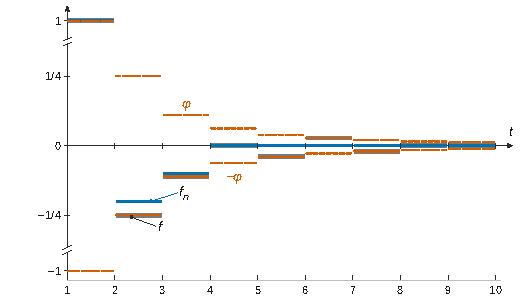
\includegraphics{figures/q20-escalier-domination.pdf}
\caption*{Figure 3 --- Pour k = 2 et n = 10, la fonction en escalier f\_n (bleu),
sa limite simple f (gris) et la domination −φ ≤ f\_n ≤ φ avec φ(t) =
1/⌊t⌋\^{}k (tirets)}
\end{figure}

\textbf{Conclusion.} Par le théorème de convergence dominée,
\equationajustee{q_n(k)=\int_1^{+\infty}f_n\xrightarrow[n\to+\infty]{}\int_1^{+\infty}f.}
Comme \(f\) est intégrable,
\equationajustee{\begin{aligned}
\int_1^{+\infty}f&=\lim_{M\to+\infty}\int_1^{M+1}f\\
&=\lim_{M\to+\infty}\sum_{d=1}^{M}\frac{\mu(d)}{d^k}\\
&=\ell.
\end{aligned}}
Donc \textbf{la suite \((q_n(k))_{n\in{\mathbb{N}}^*}\) converge} et
\equationajustee{\boxed{\lim_{n\to+\infty}q_n(k)=\sum_{d=1}^{+\infty}\frac{\mu(d)}{d^k}.}}

\hypertarget{partie-4-calcul-de-la-somme-sum_d1inftyfracmuddk}{%
\section{\texorpdfstring{Partie 4 : Calcul de la somme \(\sum_{d=1}^{+\infty}\frac{\mu(d)}{d^k}\)}{Partie 4 : Calcul de la somme \textbackslash sum\_\{d=1\}\^{}\{+\textbackslash infty\}\textbackslash frac\{\textbackslash mu(d)\}\{d\^{}k\}}}\label{partie-4-calcul-de-la-somme-sum_d1inftyfracmuddk}}

\hypertarget{question-21}{%
\subsection{Question 21}\label{question-21}}

\textbf{Inclusions.} \(F_N\subset E_N\) par définition. Si \((i,j)\in E_N\), alors \(1\le i,j\le N\le N^2\) et \(ij\le N^2\), donc \((i,j)\in F_{N^2}\) :
\equationajustee{\boxed{F_N\subset E_N\subset F_{N^2}.}}

\begin{figure}[H]
\centering
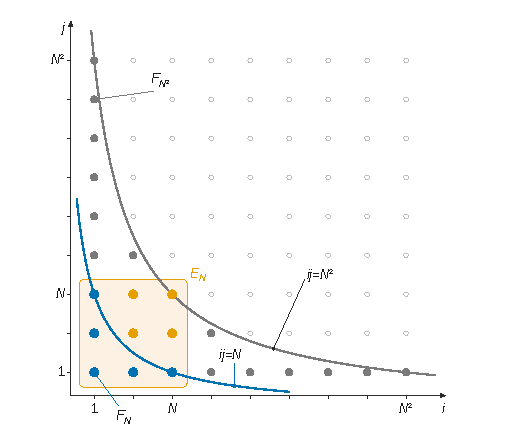
\includegraphics{figures/q21-domaines-fn-en.pdf}
\caption*{Figure 4 --- Pour N = 3, F\_N (bleu) sous l'hyperbole ij = N, le carré
E\_N (orange pour E\_N privé de F\_N) et F\_N² (gris) sous l'hyperbole
ij = N², qui passe par le coin (N, N)}
\end{figure}

\textbf{Réindexation.} L'application \((m,d)\mapsto(d,m/d)\) est une bijection de \(\{(m,d):1\le m\le N,\ d\mid m\}\) sur \(F_N\), de réciproque \((i,j)\mapsto(ij,i)\). Donc
\equationajustee{\begin{aligned}
S_N&=\sum_{m=1}^{N}\sum_{d\mid m}|u_d|\,v_{m/d}\\
&=\sum_{(i,j)\in F_N}|u_i|v_j.
\end{aligned}}

\textbf{Convergence.} Les termes sont positifs et \(F_N\subset F_{N+1}\), donc \((S_N)\) est croissante. Posons
\equationajustee{\begin{aligned}
T_N&=\sum_{(i,j)\in E_N}|u_i|v_j\\
&=\left(\sum_{i=1}^{N}|u_i|\right)\left(\sum_{j=1}^{N}v_j\right).
\end{aligned}}
Posons aussi \(U=\sum_{i\ge1}\frac{|\mu(i)|}{i^s}\) et \(V=\sum_{j\ge1}\frac1{j^s}\). Ces séries convergent, car \(|u_i|\le v_i=i^{-s}\) et \(s>1\).

On a \(S_N\le T_N\le UV\). Croissante et majorée, \textbf{\((S_N)\) converge}, vers une limite \(L\).

\textbf{Identité.} Les inclusions et la positivité des termes donnent \(S_N\le T_N\le S_{N^2}\). Comme \(S_{N^2}\to L\) (suite extraite), on a \(T_N\to L\) ; mais \(T_N\to UV\). Donc \(L=UV\) :
\equationajustee{\boxed{\begin{aligned}{}&\sum_{m=1}^{+\infty}\left(\sum_{d\mid m}|u_d|\,v_{m/d}\right)\\
&\quad=\left(\sum_{i=1}^{+\infty}\frac{|\mu(i)|}{i^s}\right)\left(\sum_{j=1}^{+\infty}\frac1{j^s}\right).
\end{aligned}}}

\hypertarget{question-22}{%
\subsection{Question 22}\label{question-22}}

La même bijection (sur des sommes finies) donne
\equationajustee{\sum_{m=1}^{N}\sum_{d\mid m}u_dv_{m/d}=\sum_{(i,j)\in F_N}u_iv_j,}
et, en développant le produit de deux sommes finies,
\equationajustee{\begin{aligned}{}&\left(\sum_{i=1}^{N}u_i\right)\left(\sum_{j=1}^{N}v_j\right)\\
&\quad=\sum_{(i,j)\in E_N}u_iv_j.
\end{aligned}}
La différence vaut \(\sum_{(i,j)\in E_N\setminus F_N}u_iv_j\). Par l'inégalité triangulaire (avec \(v_j>0\)) :
\equationajustee{\boxed{\begin{aligned}{}&\left|\left(\sum_{i=1}^{N}u_i\right)\left(\sum_{j=1}^{N}v_j\right)-\sum_{m=1}^{N}\left(\sum_{d\mid m}u_dv_{m/d}\right)\right|\\
&\quad\le\sum_{(i,j)\in E_N}|u_i|v_j-\sum_{(i,j)\in F_N}|u_i|v_j.
\end{aligned}}}

Le majorant vaut \(T_N-S_N\), qui tend vers \(UV-UV=0\) (question 21). Les séries \(\sum u_i\) et \(\sum v_j\) convergent (absolument), donc le produit de leurs sommes partielles tend vers \(\left(\sum u_i\right)\left(\sum v_j\right)\). Par suite, \(\sum_{m=1}^{N}\sum_{d\mid m}u_dv_{m/d}\) converge vers la même limite.

Enfin, pour \(d\mid m\),
\equationajustee{u_dv_{m/d}=\frac{\mu(d)}{d^s}\cdot\frac{d^s}{m^s}=\frac{\mu(d)}{m^s},}
d'où
\equationajustee{\boxed{\begin{aligned}{}&\sum_{m=1}^{+\infty}\frac1{m^s}\left(\sum_{d\mid m}\mu(d)\right)\\
&\quad=\left(\sum_{i=1}^{+\infty}\frac{\mu(i)}{i^s}\right)\left(\sum_{j=1}^{+\infty}\frac1{j^s}\right).
\end{aligned}}}

\hypertarget{question-23}{%
\subsection{Question 23}\label{question-23}}

Si \(m=1\), la somme vaut \(\mu(1)=1\).

Si \(m\ge2\), écrivons \(m=\prod_{i=1}^{r}q_i^{\alpha_i}\) avec \(r\ge1\), les \(q_i\) premiers distincts et \(\alpha_i\ge1\).

Un diviseur \(d\) de \(m\) tel que \(\mu(d)\ne0\) est sans facteur carré, et ses facteurs premiers divisent \(m\).

Il s'écrit donc \(d=\prod_{i\in I}q_i\) pour une unique partie \(I\subset[\![1;r]\!]\), et \(\mu(d)=(-1)^{\operatorname{Card}I}\).

Réciproquement, chaque tel produit divise \(m\). Les autres diviseurs vérifient \(\mu(d)=0\). Donc
\equationajustee{\begin{aligned}
\sum_{d\mid m}\mu(d)&=\sum_{I\subset[\![1;r]\!]}(-1)^{\operatorname{Card}I}\\
&=\sum_{j=0}^{r}\binom rj(-1)^j\\
&=(1-1)^r=0.
\end{aligned}}
Finalement :
\equationajustee{\boxed{\sum_{d\mid m}\mu(d)=\begin{cases}1&\text{si }m=1\\0&\text{sinon.}\end{cases}}}

\hypertarget{question-24}{%
\subsection{Question 24}\label{question-24}}

Soit \(s>1\). Par la question 23, le membre de gauche de la question 22 se réduit au terme \(m=1\), qui vaut \(1\). Donc \(\left(\sum_{i\ge1}\frac{\mu(i)}{i^s}\right)\zeta(s)=1\).

Comme \(\zeta(s)\ge1>0\) (premier terme \(1\), termes positifs), on peut diviser. Pour tout \(s>1\) :
\equationajustee{\boxed{\sum_{i=1}^{+\infty}\frac{\mu(i)}{i^s}=\frac{1}{\zeta(s)}.}}

\hypertarget{question-25}{%
\subsection{Question 25}\label{question-25}}

Soit \(k\ge2\). Par la question 20, \(\lim_{n\to+\infty}q_n(k)=\sum_{d\ge1}\frac{\mu(d)}{d^k}\). Par la question 24 avec \(s=k>1\), cette somme vaut \(\frac1{\zeta(k)}\) :
\equationajustee{\boxed{\lim_{n\to+\infty}q_n(k)=\frac{1}{\zeta(k)}.}}
Avec les valeurs de la question 14 :
\equationajustee{\boxed{\begin{aligned}
\lim_{n\to+\infty}q_n(2)&=\frac{6}{\pi^2}\approx0{,}608,\\
\lim_{n\to+\infty}q_n(4)&=\frac{90}{\pi^4}\approx0{,}924.
\end{aligned}}}

\end{document}
